\documentclass[11pt, a4paper]{article}		% general format


%%%% Charset
\usepackage[utf8]{inputenc}					% use utf8					
\usepackage[russian]{babel}					% use russian font


%%%% Math
\usepackage{amsmath}						% Amer­i­can Math­e­mat­i­cal So­ci­ety (AMS) math fa­cil­i­ties
\usepackage{amsfonts}						% fonts from the AMS
\usepackage{amssymb}						% additional math symbols


%%%% Graphics
\usepackage{graphicx}


\author{Дедков Сергей}
\title{Отчет по лабораторной работе №5 :\\ Инструмент тестов на проникновение metasploit}
\date{2015}

%---------------------------------------------------------

\begin{document}
\maketitle
\tableofcontents
\newpage

%---------------------------------------------------------


\section{Цель работы}

Изучить варианты использования metasploit.



%---------------------------------------------------------

\section{Ход работы, теория}


%---------------------------------------------------------

\subsection{Используя документацию изучить основные понятия auxiliary, payload, exploit, shellcode,	nop, encoder}

\begin{itemize}
\item auxiliary - сканер, который использует уязвимости системы, для полкучения сведений о это системе.

\item payload - полезная нагрузка - в компьютерной безопасности относится к той части вредоносных программ, который выполняет вредоносные действия. При анализе вредоносных программ, таких как черви, вирусы и троянские программы, это относится к вредным результатам данного программного обеспечения. Примеры полезных нагрузок включают разрушение данных, сообщений оскорбительного текста или ложных сообщений электронной почты, отправляемых с большим количеством людей. Таким образом, полезная нагрузка относится к фактическому назначению сообщение в коробке передач.

\item exploit (англ. exploit — использовать) - это общий термин в сообществе компьютерной безопасности для обозначения фрагмента программного кода который, используя возможности предоставляемые ошибкой, отказом или уязвимостью, ведёт к повышению привилегий или отказу в обслуживании компьютерной системы.

\item shellcode (англ. shellcode - код оболочки) - это двоичный исполняемый код, который обычно передаёт управление консоли, например \verb'’/bin/sh’' Unix shell, command.com в MS-DOS и cmd.exe в операционных системах Microsoft Windows. Код оболочки может быть использован как полезная нагрузка эксплойта, обеспечивая взломщику доступ к командной оболочке (англ. shell) в компьютерной системе.

\item nop (сокращение от англ.: «No OPeration») - инструкция процессора на языке ассемблера, или команда протокола, которая предписывает ничего не делать.

\item encoder - это устройство преобразующее линейное или угловое перемещение в последовательность сигналов, позволяющих определить величину перемещения. Т.о. можно выделить линейные и поворотные энкодеры.

\end{itemize}

%---------------------------------------------------------

\subsection{Запуск msfconsole}

Запустим msfconsole и узнаем список допустимых команд (help).

При вводе команды help, можно посмотреть список доступных команд. Перечислять все не имеет смысле, какие-то описаны ниже, а какие-то мы уже знаем.

Фреймворк Metasploit обладает тремя рабочими окружениями: msfconsole, msfcli и msfweb. Основным и наиболее предпочтительным из трех перечисленных вариантов является первый - msfconsole. Это окружение представляет из себя эффективный интерфейс командной строки со своим собственным набором команд и системным окружением.

%---------------------------------------------------------

\subsection{Базовые команды}

Базовыми командами являются search (поиск по имени, типу, автору и др.), info, load, use.

\begin{itemize}
\item search <keyword> - запустив команду search без указания ключевых слов, выводится список всех доступных эксплоитов. Если значение <keyword> имеет имя определенного сплоита, то этой командой ищем такой в базе данных системы.

\item info <type> <name> - если нужна конкретная и полная информация о каком-либо эксплоите или payload’е, можно применить команду info. Например, нужно подробное описание payload’а winbind. Тогда необходимо набрать в командной строке info payload winbind и получить справочную информацию по нему.

\item load - команда используется для загрузки плагинов.

\item use <exploit\_name> - команда говорит Фреймворку Metasploi запустить эксплоит с указанным конкретным именем

\end{itemize}

%---------------------------------------------------------

\subsection{Команды по работе с эксплоитом}

Для работы с эксплоитом используются следующие команды:

\begin{itemize}

\item show exploits - указав команду show exploits, получим список всех доступных на данный момент эксплоитов. Имеются версии последних под различные платформы и приложения, включая Windows, Linux, IIS, Apache и так далее. Это поможет понять работу фреймворка Metasploit и почувствовать его гибкость и эффективность.

\item show options - набрав в командной строке show options, будет выведет список опций, которые можно использовать. Каждый эксплоит или payload имеет свой собственный набор опций, который можно использовать при работе с ними.

\item exploit - запускает эксплоит. Есть другая версия этой команды - rexploit, которая перезагружает код запущенного эксплоита и запускает его вновь. Эти две команды помогают работать с эксплоитами с минимальными усилиями, без перезапуска консоли.

\item set RHOST <hostname\_or\_ip> - указываем этой командой Metasploit определенный хост в сети для его изучения. Хост можно задать как по его имени, так и по IP-адресу.

\item set RPORT <host\_port> - задает для Metasploit порт удаленной машины, по которому фреймворк должен подключиться к указанному хосту

\item set payload <generic/shell\_bind\_tcp> - команда указывает имя payload’а, который будет использоваться.

\item  set LPORT <local\_port> - задаем номер порта для payload’а на сервере, на котором был выполнен эксплоит. Это важно, так как номер этого порта открыт именно на сервере (он не может быть использован никакими другими службами этого сервера и не резервируется для административных нужд). Советую назначать такой номер из набора четырех случайных цифр, порядок которых начинается с 1024. И тогда у вас все будет хорошо. Также стоит упомянуть, что необходимо менять номер порта каждый раз, когда успешно запущен эксплоит на удаленной машине.

\end{itemize}


%---------------------------------------------------------

\subsection{Команды по работе с БД}

\begin{itemize}

\item db\_connect - подключение к базе данных.

\item db\_status - проверка состояния базы данных.

\item db\_host - просмотр списка хостов в файле базы данных.

\item db\_del\_host - удалить какой-либо хост из базы данных.

\end{itemize}


%---------------------------------------------------------

\subsection{GUI оболочка Armitage}

Графическая оболочка для набора утилит и библиотеки эксплоитов Metasploit. Armitage позволяет в наглядном виде представить все этапы атаки, включая: сканирование узлов сети, анализ защищенности обнаруженных ресурсов, выполнение эксплоитов и получение полного контроля над уязвимой системой. Все функции программы структурированы и легкодоступны из меню и вкладок программы, даже для начинающего исследователя компьютерной безопасности.

Запустим и протестируем работу Armitage. Укажем начальные параметры, как на рисунке 1. Далее жмем Connect.

\begin{figure}[h!]
\centering
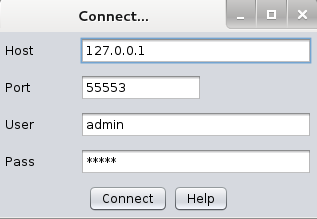
\includegraphics[scale=0.8]{res/armitage}
\caption{Настройки подключения к armitage}
\end{figure}


После запуска введем ip атакуемой машины. Проведем эксперимент из пункта 2.2.1. Для этого в боковом меню найдем необходимую auxiliary (vnc\_login) и укажем настройки. Далее нажимаем Launch. Результат выполнения успешен и представлен на рисунке 2.


\begin{figure}[h!]
\centering
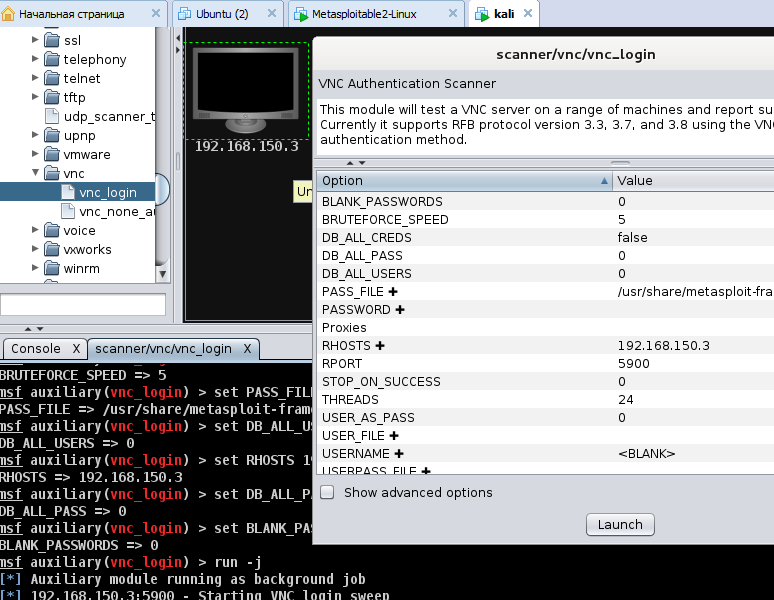
\includegraphics[scale=0.8]{res/armitage_settings}
\caption{Настройки подключения к armitage}
\end{figure}

%---------------------------------------------------------

\subsection{GUI веб-клиент}



%---------------------------------------------------------

\section{Ход работы, практика}

%---------------------------------------------------------

\subsection{Подключиться к VNC-серверу, получить доступ к консоли}










\end{document}